\documentclass{article}
\title{Homework - Biostatistics \bf{ Ducks }}
\date{Academic Year 2012/2013}
\usepackage[english]{babel}
\usepackage[cp1250]{inputenc}
\usepackage{hyperref}
\usepackage{enumerate}
\usepackage[cm,empty]{fullpage}
\usepackage[pdftex]{graphicx,color}
\usepackage{Sweave}
\begin{document}
\maketitle{}
\section{ Data about the group }{\bf Group members : }Donald Duck, Daisy Duck, Scrooge McDuck, Gladstone Gander, Elvira Grandma Duck Coot\\{\bf Due date : 8th of October 2012 }\\{\bf Sources : }Book\\{\bf Template to use : Descriptive.doc }\\\section{ Assignment }Answer to the following questions \\\begin{itemize}
\item Calculate the mean of the following data:  
6,-3,-4,4\item Calculate the standard deviation of the following data:  
4,7,7,6 
\item Data for the  variable nn are represented graphically. Determine (approximately) the mean and the standard deviation of the variable.\\ 
\begin{tabular}{c}
\resizebox{50mm}{!}{
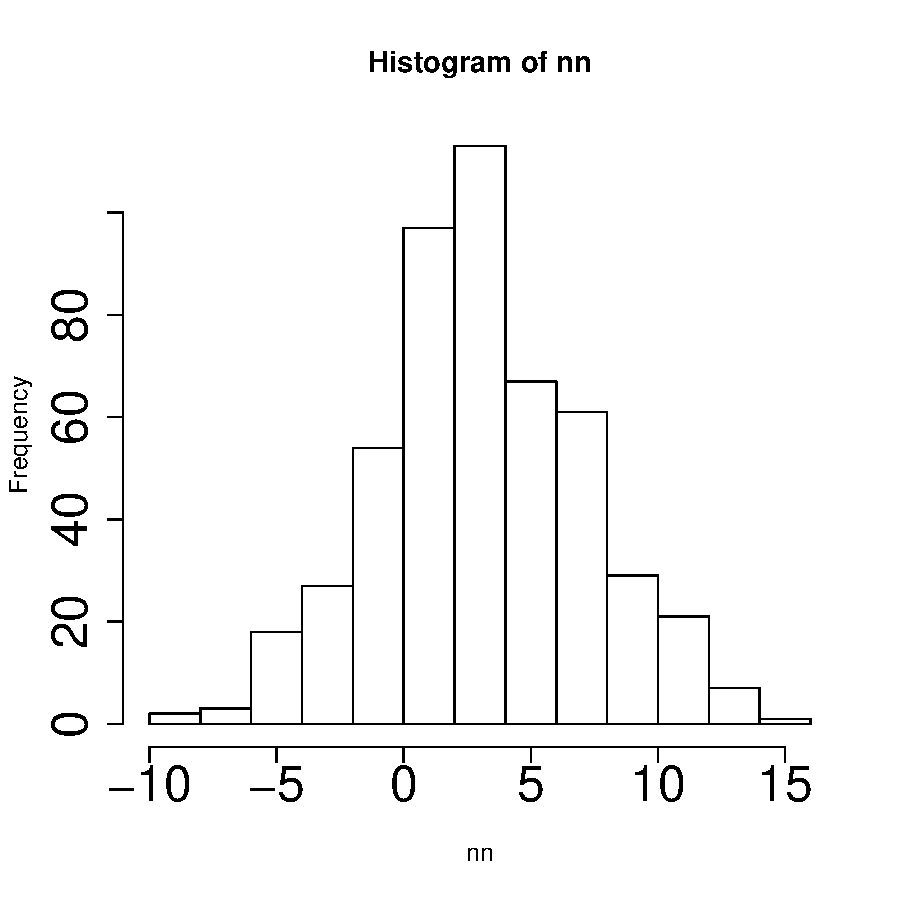
\includegraphics{Ducks-003}
}
\end{tabular} 
\end{itemize}
\vspace{\baselineskip} {\bf  }\newpage
\end{document}
